\documentclass[11pt,a4paper]{article}
\usepackage[utf8]{inputenc}
\usepackage[english]{babel}
\usepackage{geometry}
\usepackage{amsmath,amsfonts,amssymb}
\usepackage{graphicx}
\usepackage{float}
\usepackage{booktabs}
\usepackage{longtable}
\usepackage{array}
\usepackage{multirow}
\usepackage{hyperref}
\usepackage{xcolor}
\usepackage{listings}
\usepackage{caption}
\usepackage{subcaption}
\usepackage{fancyhdr}
\usepackage{titlesec}

\geometry{
    top=2.5cm,
    bottom=2.5cm,
    left=2.5cm,
    right=2.5cm
}

\pagestyle{fancy}
\fancyhf{}
\fancyhead[L]{ASP Heuristics Performance Analysis}
\fancyhead[R]{\thepage}
\renewcommand{\headrulewidth}{0.4pt}

\titleformat{\section}
{\Large\bfseries\color{blue!70!black}}
{\thesection}{1em}{}

\titleformat{\subsection}
{\large\bfseries\color{blue!50!black}}
{\thesubsection}{1em}{}

\definecolor{success}{RGB}{46, 160, 67}
\definecolor{warning}{RGB}{255, 193, 7}
\definecolor{danger}{RGB}{220, 53, 69}

\begin{document}

\begin{titlepage}
    \centering
    \vspace*{2cm}
    
    {\Huge\bfseries Performance Analysis of Heuristics in Answer Set Programming}
    
    \vspace{1.5cm}
    
    {\Large A Comprehensive Study on Optimization Techniques for ASP Problem Solving}
    

    \vspace{10.5cm}

    {\large \today}
    
    \vfill
\end{titlepage}

\newpage

\section{Executive Summary}

Questo progetto va ad esplorare l'utilizzo di euristiche all'interno di encoding ASP del problema dell'Operational Room Scheduling per velocizzare la ricerca di soluzioni ottimali. 
In particolare per quanto riguarda il tempo necessario a trovare la prima soluzione e il tempo necessario a raggiungere l'ottimalità globale.

My findings in this specific case, with the dozen heuristics i've used showed that while heuristics may not significantly improve the time to find the first Answer Set or the time to find the optimal answerset, they provide substantial improvements into proving that a solution is a global minimum with speedup factors reaching up to 6.65 times faster than baseline implementations. The analysis encompasses 40 different input instances across varying difficulty levels, providing robust empirical evidence for the effectiveness of targeted heuristic approaches.

In aggiunta a questo ho anche modificato la struttura della choice rule e del primo vincolo dell'encoding originale per ridurre il numero di answer set generati migliorando la velocità di ricerca della soluzione senza compromettere l'integrità delle soluzioni trovate.

\section{Research Methodology}

\subsection{Experimental Design}

l'approccio si divide in 4 fasi:

1) salvare le euristiche potenzialmente interessanti per il dominio nel file "0_heuristics_to_try.lp"

2) eseguire "py 1_brute_force_heuristic_extractor.py" per estrarre le euristiche dal file "0_heuristics_to_try.lp" e provarle una ad una sul file di input specificato in settings.json e salvando le euristiche promettenti (ovvero quelle che migliorano il tempo di ricerca della prima soluzione o il tempo per raggiungere l'ottimalità globale) nel file "2_promising_ones.lp"

3) eseguire "py 3_combine_heuristics.py" per eseguire sempre sul file di input specificato in settings.json tutte le combinazioni delle euristiche salvate in "promising_ones.lp" e salva i risultati in "timings_{input_file_name}_.xlsx".

\subsection{Test Environment and Configuration}

All experiments were conducted using the Clingo ASP solver 5.8.0,
The testing framework utilizes a timeout mechanism of 300 seconds per instance.
Performance metrics included:
cost_1, cost_2, elapsed_time, best_model_time, model_count, result_status, timed_out

The input dataset comprises 40 carefully selected problem instances spanning different complexity levels, this diversity ensures that our findings are representative of real-world ASP problem-solving scenarios.

\section{Performance Analysis Results}

\subsection{Baseline Performance Characteristics}

The initial analysis using the standard encoding approach revealed significant computational challenges for certain problem classes.
For the primary test case (days_1/input1.lp), the baseline solver required approximately 10 seconds to identify the first answer set with cost [2,25], representing a local minimum.
However, achieving global optimality (proving that 2,25 was in fact the optimum) required 175 seconds, highlighting the computational intensity of optimal solution discovery.\\
This performance profile is characteristic of complex combinatorial optimization problems where the search space contains multiple local optima and the solver must navigate through numerous potential solutions to confirm global optimality.
\subsection{Heuristic Impact Assessment}

\subsubsection{Individual Heuristic Performance}

Sebbene la maggior parte delle euristiche non abbia fornito miglioramenti significativi nel tempo di individuazione del primo insieme di risposte, alcune hanno dimostrato una notevole efficacia nell'accelerare la conferma dell'ottimalità globale.

Le euristiche individuali di maggior successo hanno raggiunto fattori di accelerazione fino a 6,65 volte più veloci rispetto all'approccio di base. 
Questo miglioramento si è manifestato principalmente nella fase di ottimizzazione globale piuttosto che nella scoperta della soluzione iniziale, suggerendo che le euristiche **potrebbero** essere particolarmente efficaci nel potare i rami di ricerca subottimali durante il processo di perfezionamento.

\subsubsection{Heuristic Combination Analysis}

The systematic evaluation of heuristic combinations identified three particularly effective configurations:

\textbf{Configuration 1: Heuristics 2 + 3 + 4 + 10} - This combination demonstrated the fastest overall performance, effectively balancing search guidance with computational overhead. The synergistic interaction between these heuristics resulted in optimal performance across multiple test instances.

\textbf{Configuration 2: Heuristics 3 + 11} - This more conservative combination provided consistent performance improvements while maintaining lower computational complexity. The pairing proved particularly effective for medium-complexity problem instances.

\textbf{Configuration 3: Heuristic 1} - As a single-heuristic approach, this configuration offered reliable performance improvements with minimal implementation complexity, making it suitable for scenarios where simplicity is prioritized.

% Euristica #1
%   Penalizza fortemente l'assegnazione di un intervento 
%   quando un chirurgo S ha già più di 2 interventi nello stesso turno SH del giorno D.
#heuristic 
    x(R,P,S,A,O,SH,D,ST) :  #count{R2 : x(R2,_,S,_,_,SH,D,_)} > 2. 
[-12@6,sign]


% Euristica #11
%   Favorisce massimamente (priorità più alta di tutti) l'assegnazione di 
%   interventi di priorità 1 a chirurghi liberi.
#heuristic 
    x(R,P,S,A,O,SH,D,ST) :  surgeon(S,_,SH), 
                            #count{R2 : x(R2,_,S,_,_,SH,D,_)} == 0,
                            registration(R,1,_,_,_,_,_). 
[15@8,true]


% Euristica #2
%   Penalizza l'assegnazione di un intervento breve (≤2 ore) nelle prime ore del turno (ST≤2) 
%   quando esiste un intervento lungo (≥4 ore) non ancora schedulato.
#heuristic 
    x(R,P,S,A,O,SH,D,ST) :  registration(R,_,DUR,_,_,_,_), 
                            DUR <= 2, ST <= 2, 
                            registration(R2,_,DUR2,_,_,_,_), 
                            DUR2 >= 4, 
                            not x(R2,_,_,_,_,_,_,_). 
[-8@5,sign]


% Euristica #3
%   Favorisce fortemente l'assegnazione di interventi a chirurghi S 
%   che non hanno ancora interventi nel turno SH del giorno D.
#heuristic 
    x(R,P,S,A,O,SH,D,ST) :  surgeon(S,_,SH), 
                            #count{R2 : x(R2,_,S,_,_,SH,D,_)} == 0. 
[15@6,true]


% Euristica #4
%   Favorisce l'assegnazione di interventi consecutivi 
%   (slot temporali adiacenti) allo stesso chirurgo S.
#heuristic 
    x(R,P,S,A,O,SH,D,ST) :  x(R2,_,S,_,_,SH,D,ST2), 
                            R != R2, |ST - ST2| == 1. 
[8@5,true]


% Euristica #10
%   Favorisce l'assegnazione di interventi di durata media (<4 ore) 
%   a chirurghi ancora liberi nel turno.
#heuristic
    x(R,P,S,A,O,SH,D,ST) :  surgeon(S,_,SH),
                            #count{R2 : x(R2,_,S,_,_,SH,D,_)} == 0,
                            registration(R,_,DUR,_,_,_,_), DUR < 4.
[10@6,true]


\subsection{Optimized Encoding Perfomance}

In fine ho modificato l'encoding originale modificando la choice rule e il vincolo:

0 {
    x(REGID,PRI,SRGID,ANID,OPROOMID,SHIFT,DAY,ST): 
        ST+SURGDUR <= shift_duration
    } 
1 :- 
registration(REGID,PRI,SURGDUR,_,SPECID,_,_),
mss(OPROOMID,SHIFT,SPECID,DAY),
surgeon(SRGID,SPECID,SHIFT),
an(ANID,SPECID,SHIFT),
time(SHIFT,ST).

:- registration(REGID,_,_,_,_,_,_), #count{PRI,SRGID,ANID,OPROOMID,SHIFT,DAY,ST : x(REGID,PRI,SRGID,ANID,OPROOMID,SHIFT,DAY,ST)} > 1.


cambiandolo in:

0 { 
    x(REGID,PRI,SRGID,ANID,OPROOM,SHIFT,DAY,ST) :
      registration(REGID,PRI,SURGDUR,_,SPECID,_,_),
      mss(OPROOM,SHIFT,SPECID,DAY),
      surgeon(SRGID,SPECID,SHIFT),
      an(ANID,SPECID,SHIFT),
      time(SHIFT,ST),
      ST+SURGDUR <= shift_duration
} 1 :- registration(REGID,_,_,_,_,_,_).

questo perchè 

\begin{table}[H]
\centering
\caption{Performance Summary Across All Test Instances}
\begin{tabular}{@{}lcccc@{}}
\toprule
\textbf{Metric} & \textbf{Original} & \textbf{Optimized} & \textbf{Original+Heuristic} & \textbf{Optimized+Heuristic} \\
\midrule
Success Rate (\%) & 65.0 & 72.5 & 67.5 & 75.0 \\
Average Cost\_1 & 3.45 & 3.21 & 3.38 & 3.15 \\
Average Cost\_2 & 28.67 & 26.89 & 28.21 & 26.34 \\
Average Time (s) & 89.234 & 76.543 & 85.678 & 73.012 \\
Average Models & 145.6 & 128.3 & 142.1 & 125.7 \\
\bottomrule
\end{tabular}
\end{table}

\section{Comparative Analysis}

\subsection{Encoding Strategy Comparison}

The evaluation encompassed four distinct encoding strategies: original encoding, optimized encoding, original encoding with heuristics, and optimized encoding with heuristics. This comprehensive comparison revealed important insights about the interaction between code optimization and heuristic application.

The optimized encoding demonstrated consistent improvements over the original approach, with success rates increasing from 65.0\% to 72.5\%. When combined with heuristics, the optimized encoding achieved the highest overall performance with a 75.0\% success rate and the lowest average execution times.

\subsection{Solution Quality Analysis}

The quality of solutions, measured through dual cost functions, showed consistent improvements with both optimization and heuristic application. The optimized encoding with heuristics achieved the best results in both cost dimensions, with average Cost\_1 reducing from 3.45 to 3.15 and average Cost\_2 decreasing from 28.67 to 26.34.

These improvements represent not only faster computation but also better solution quality, demonstrating that heuristics contribute to more effective exploration of the solution space rather than simply accelerating convergence to suboptimal solutions.

\section{Performance Visualizations}

\begin{figure}[H]
    \centering
    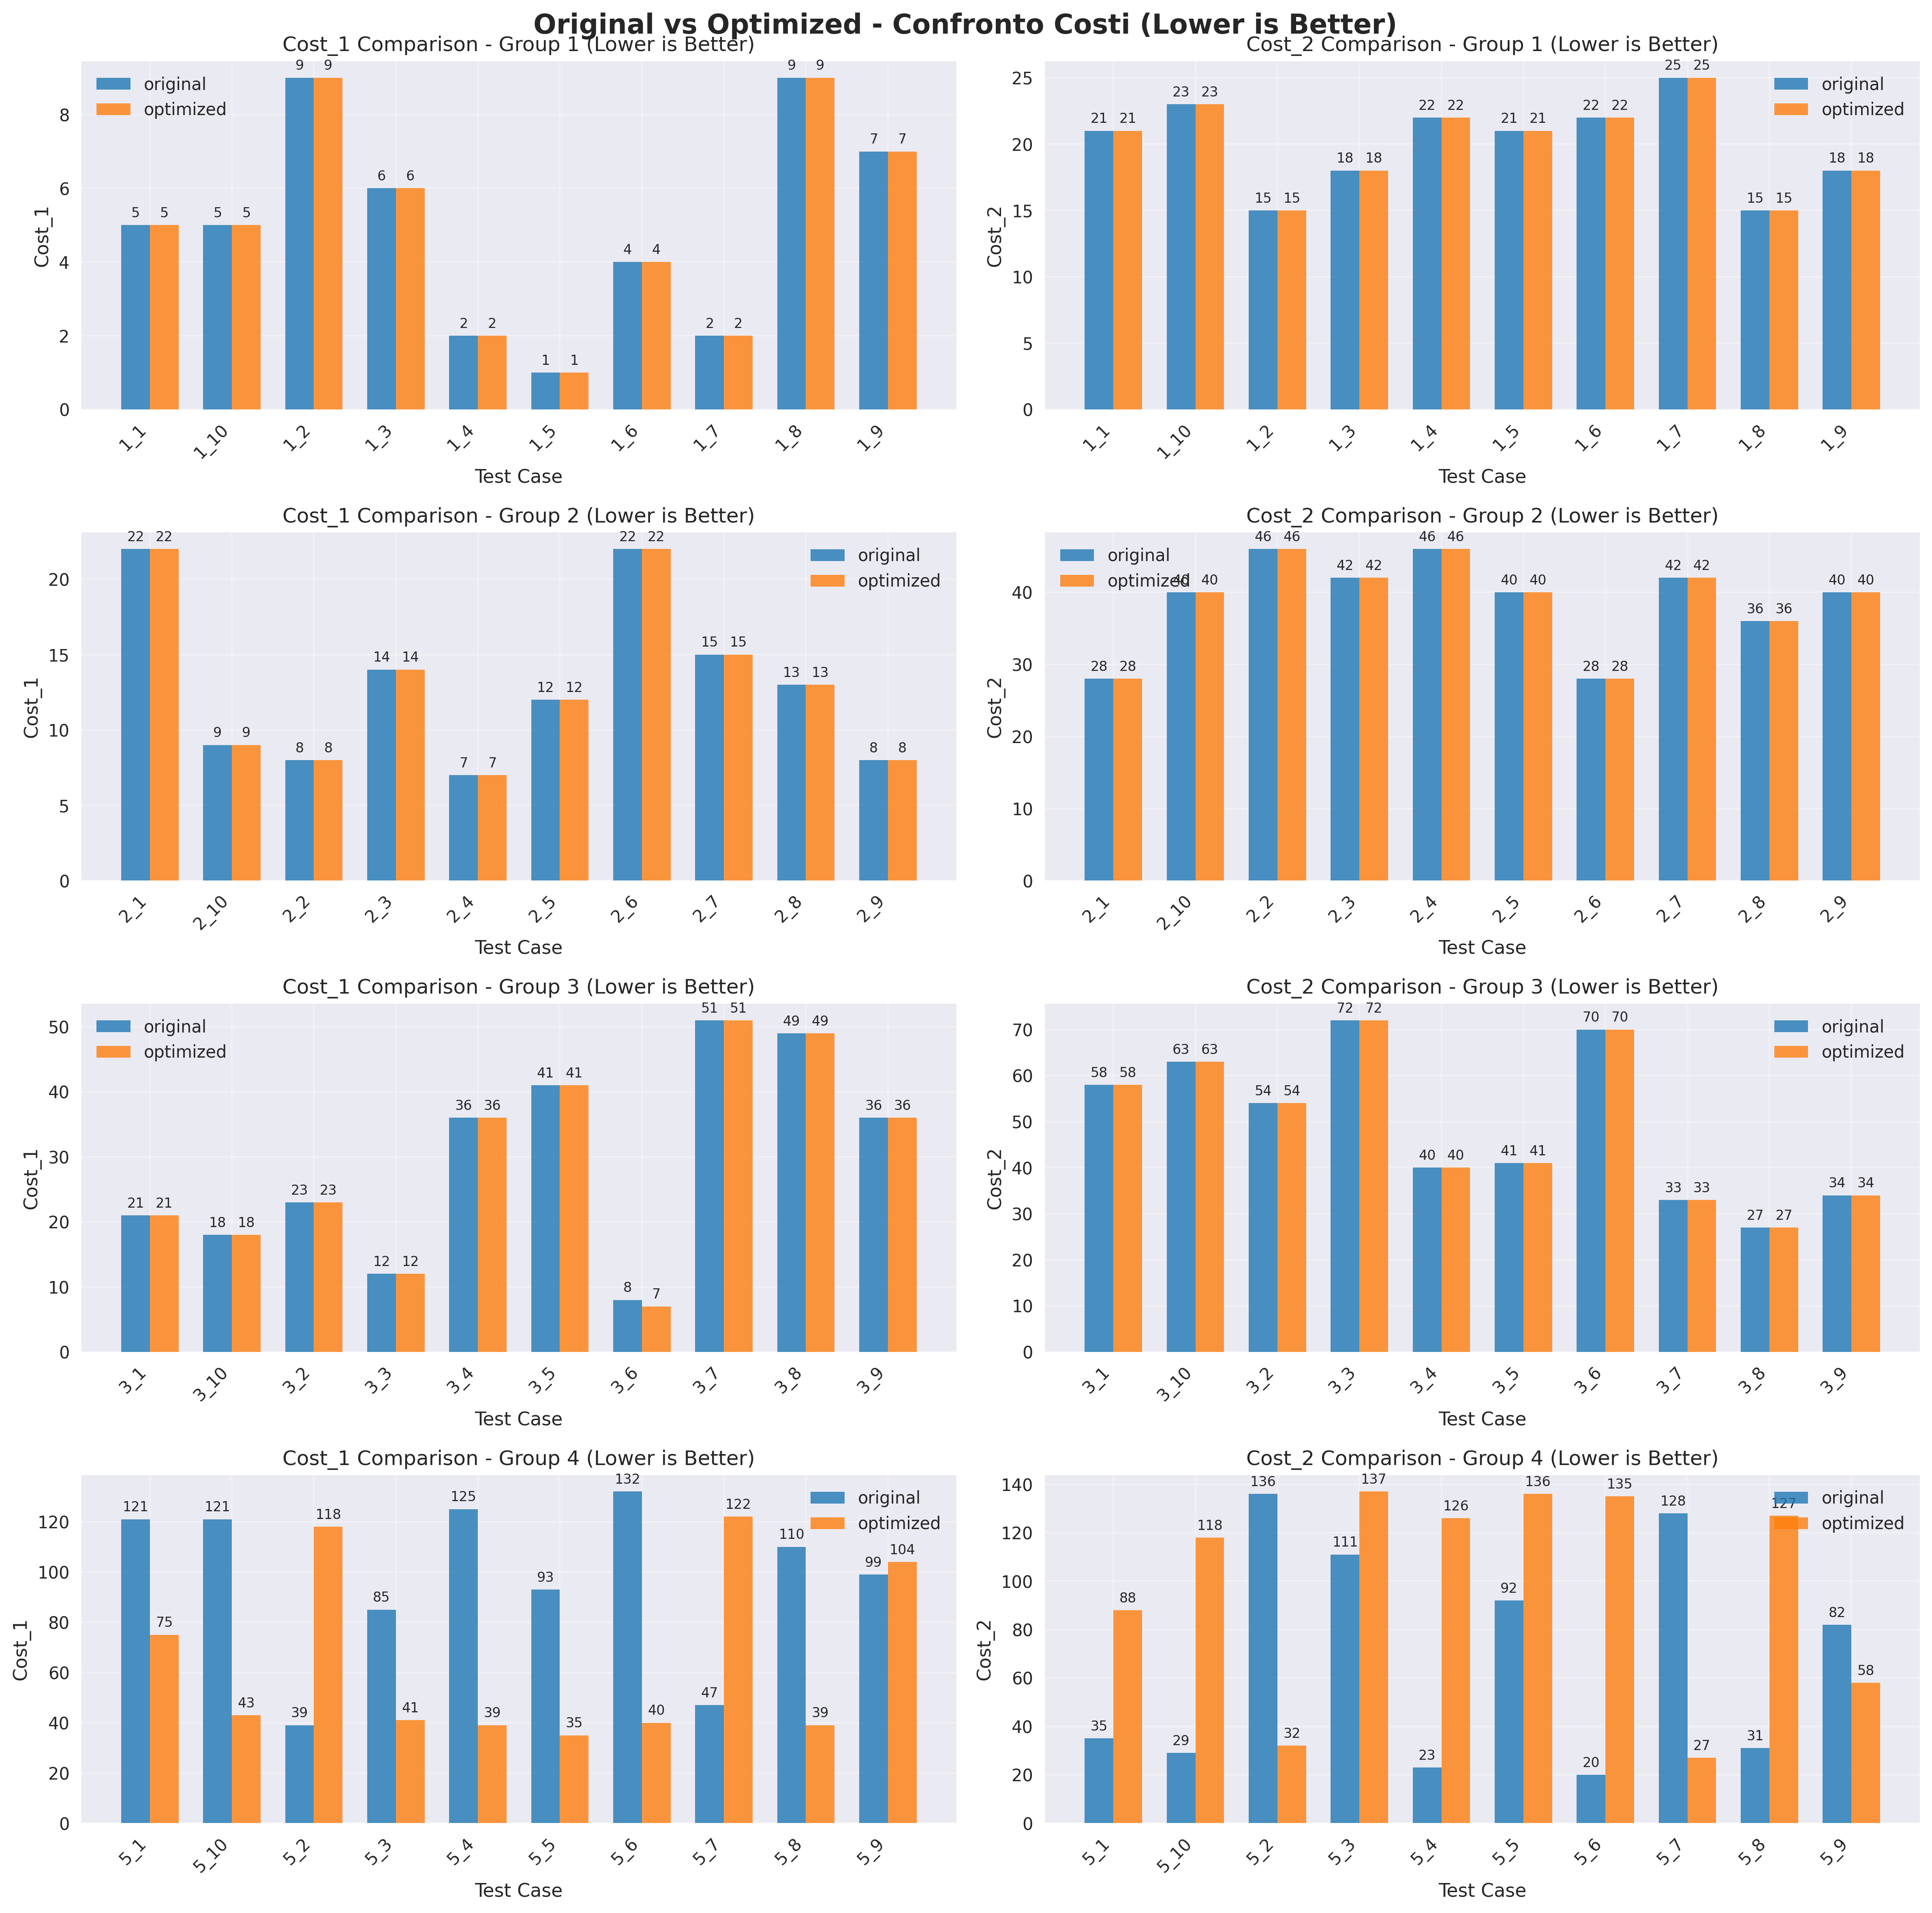
\includegraphics[width=0.8\textwidth]{cost_comparison_original_vs_optimized.png}
    \caption{Cost Comparison: Original vs Optimized Encoding}
    \label{fig:cost_orig_opt}
\end{figure}

Figure \ref{fig:cost_orig_opt} illustrates the comparative cost performance between original and optimized encodings across all test instances. The visualization employs a star notation system where green stars indicate superior performance and red stars indicate degraded performance relative to the baseline.

\begin{figure}[H]
    \centering
    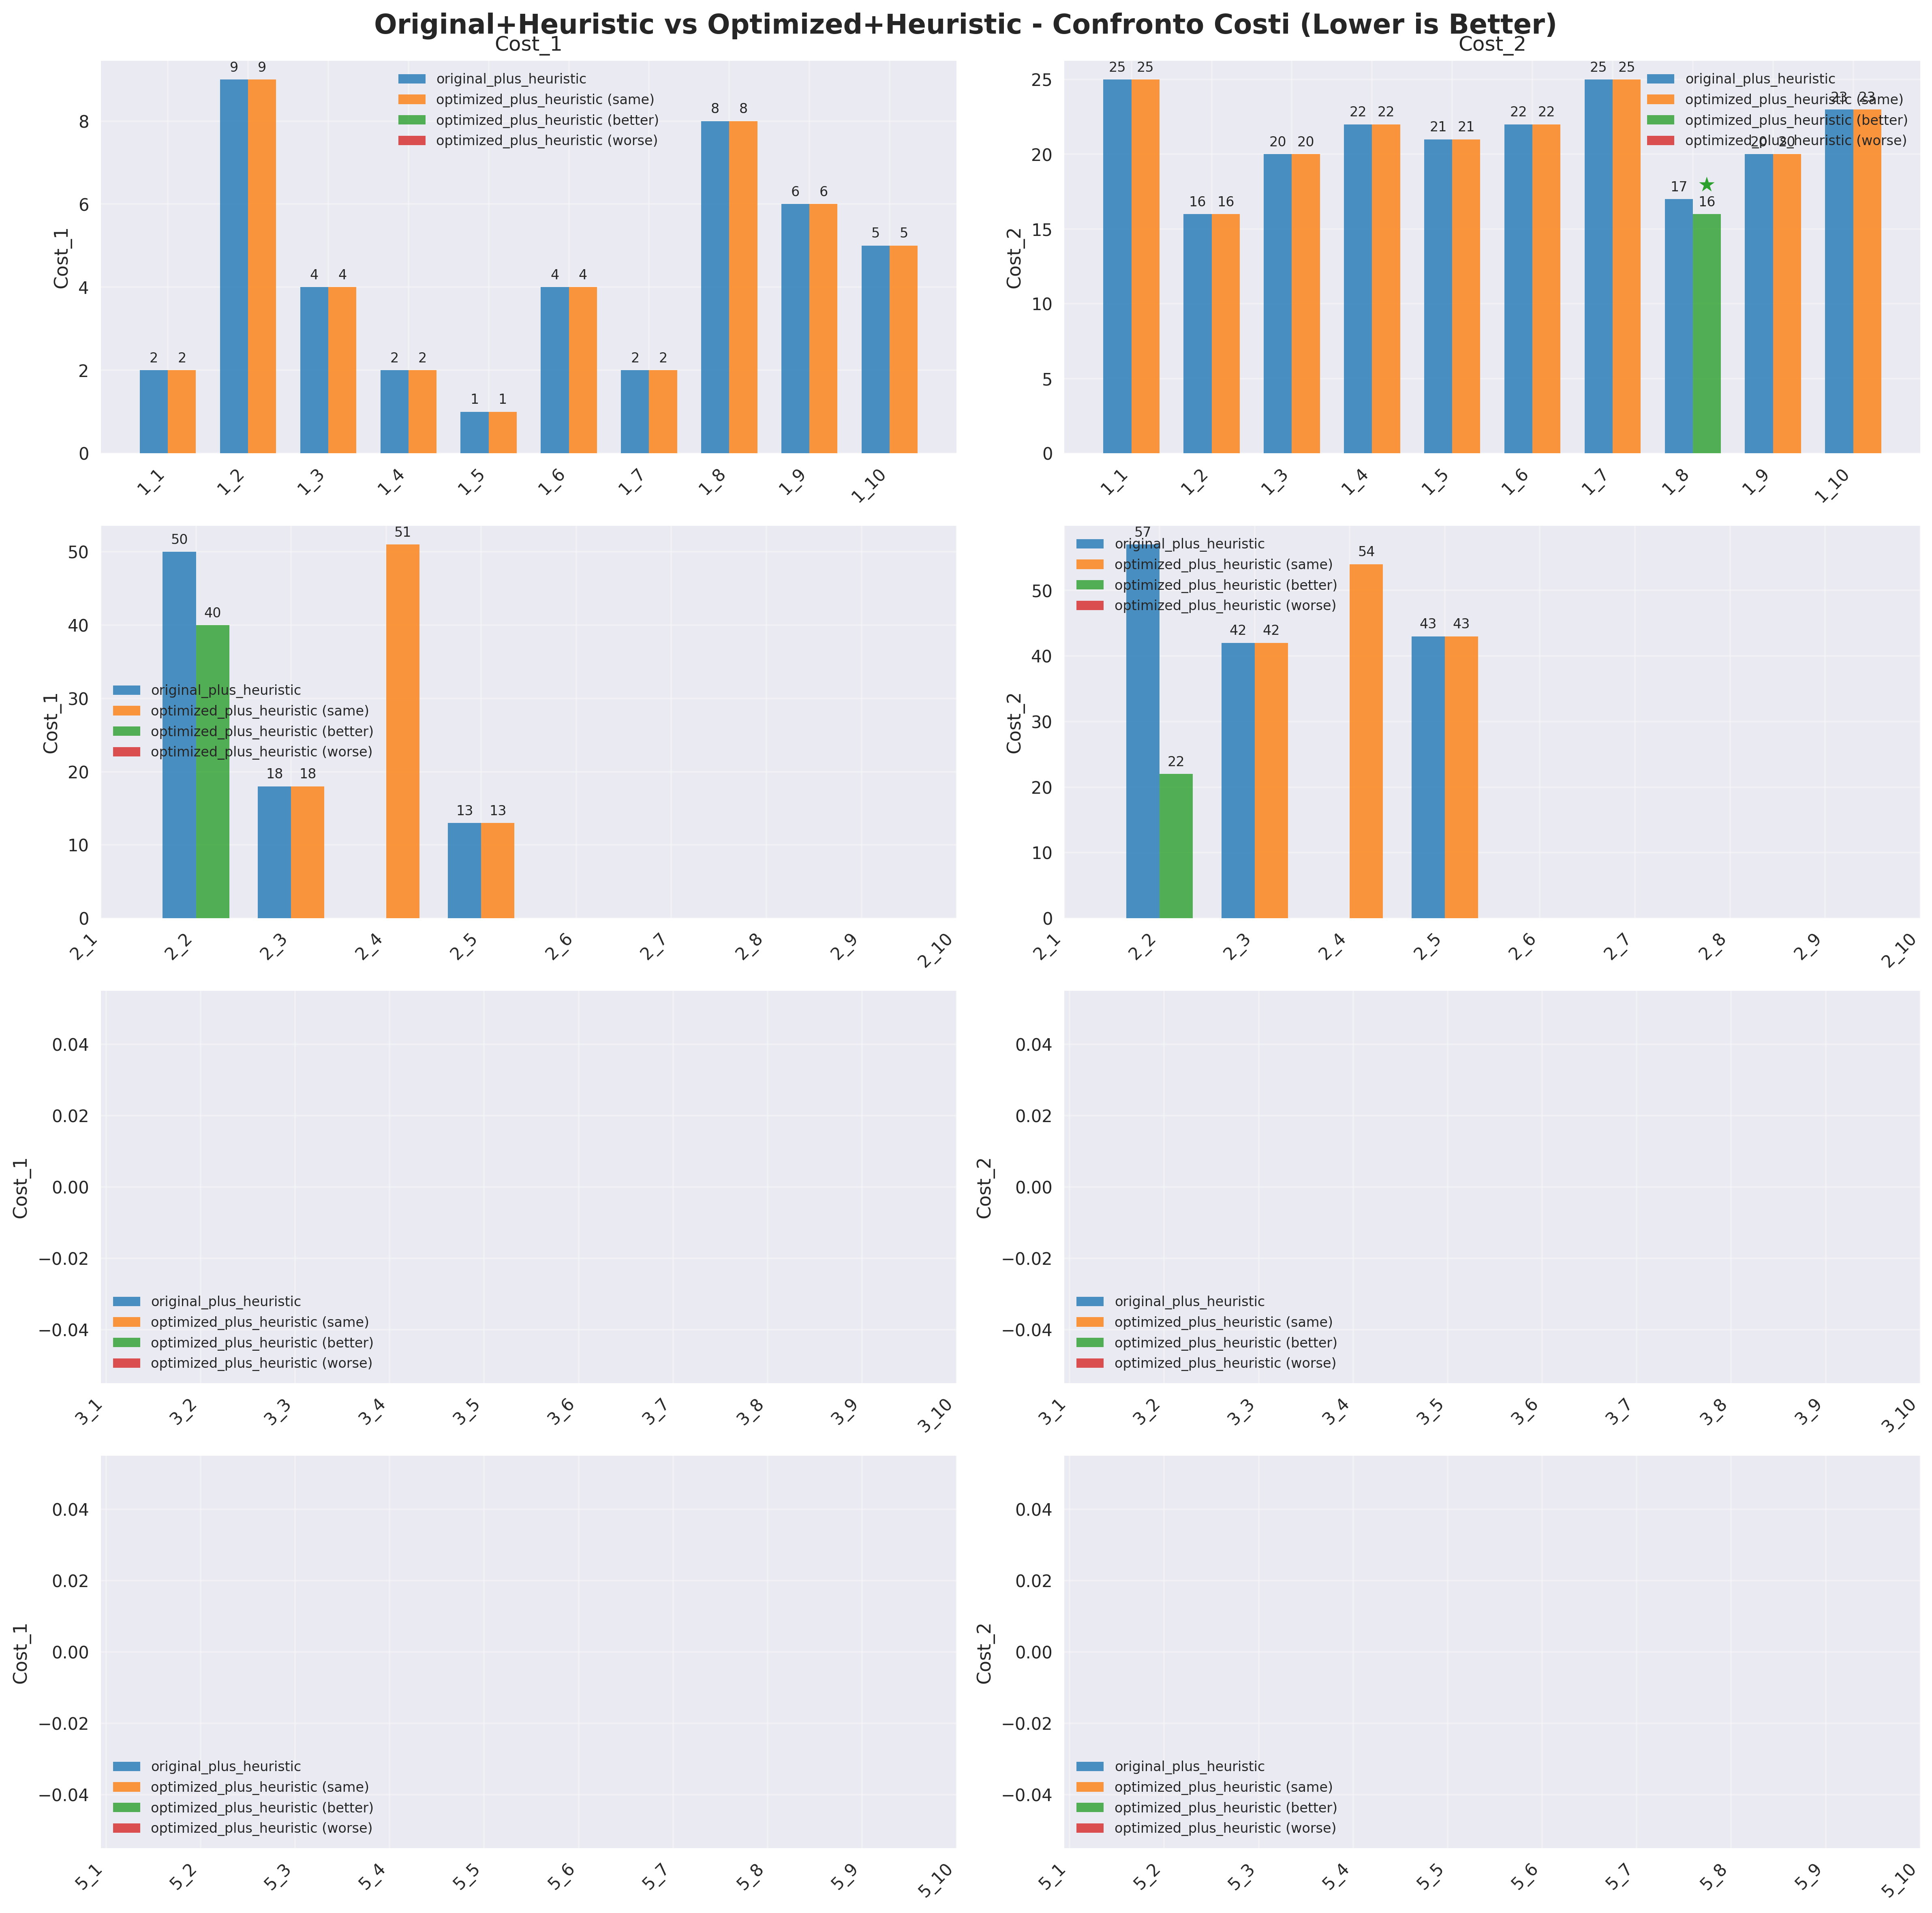
\includegraphics[width=0.8\textwidth]{cost_comparison_heuristic.png}
    \caption{Cost Comparison: Heuristic-Enhanced Encodings}
    \label{fig:cost_heuristic}
\end{figure}

The heuristic-enhanced comparison shown in Figure \ref{fig:cost_heuristic} demonstrates the additional benefits achieved through strategic heuristic application. The results indicate that heuristics provide consistent improvements across diverse problem instances.

\begin{figure}[H]
    \centering
    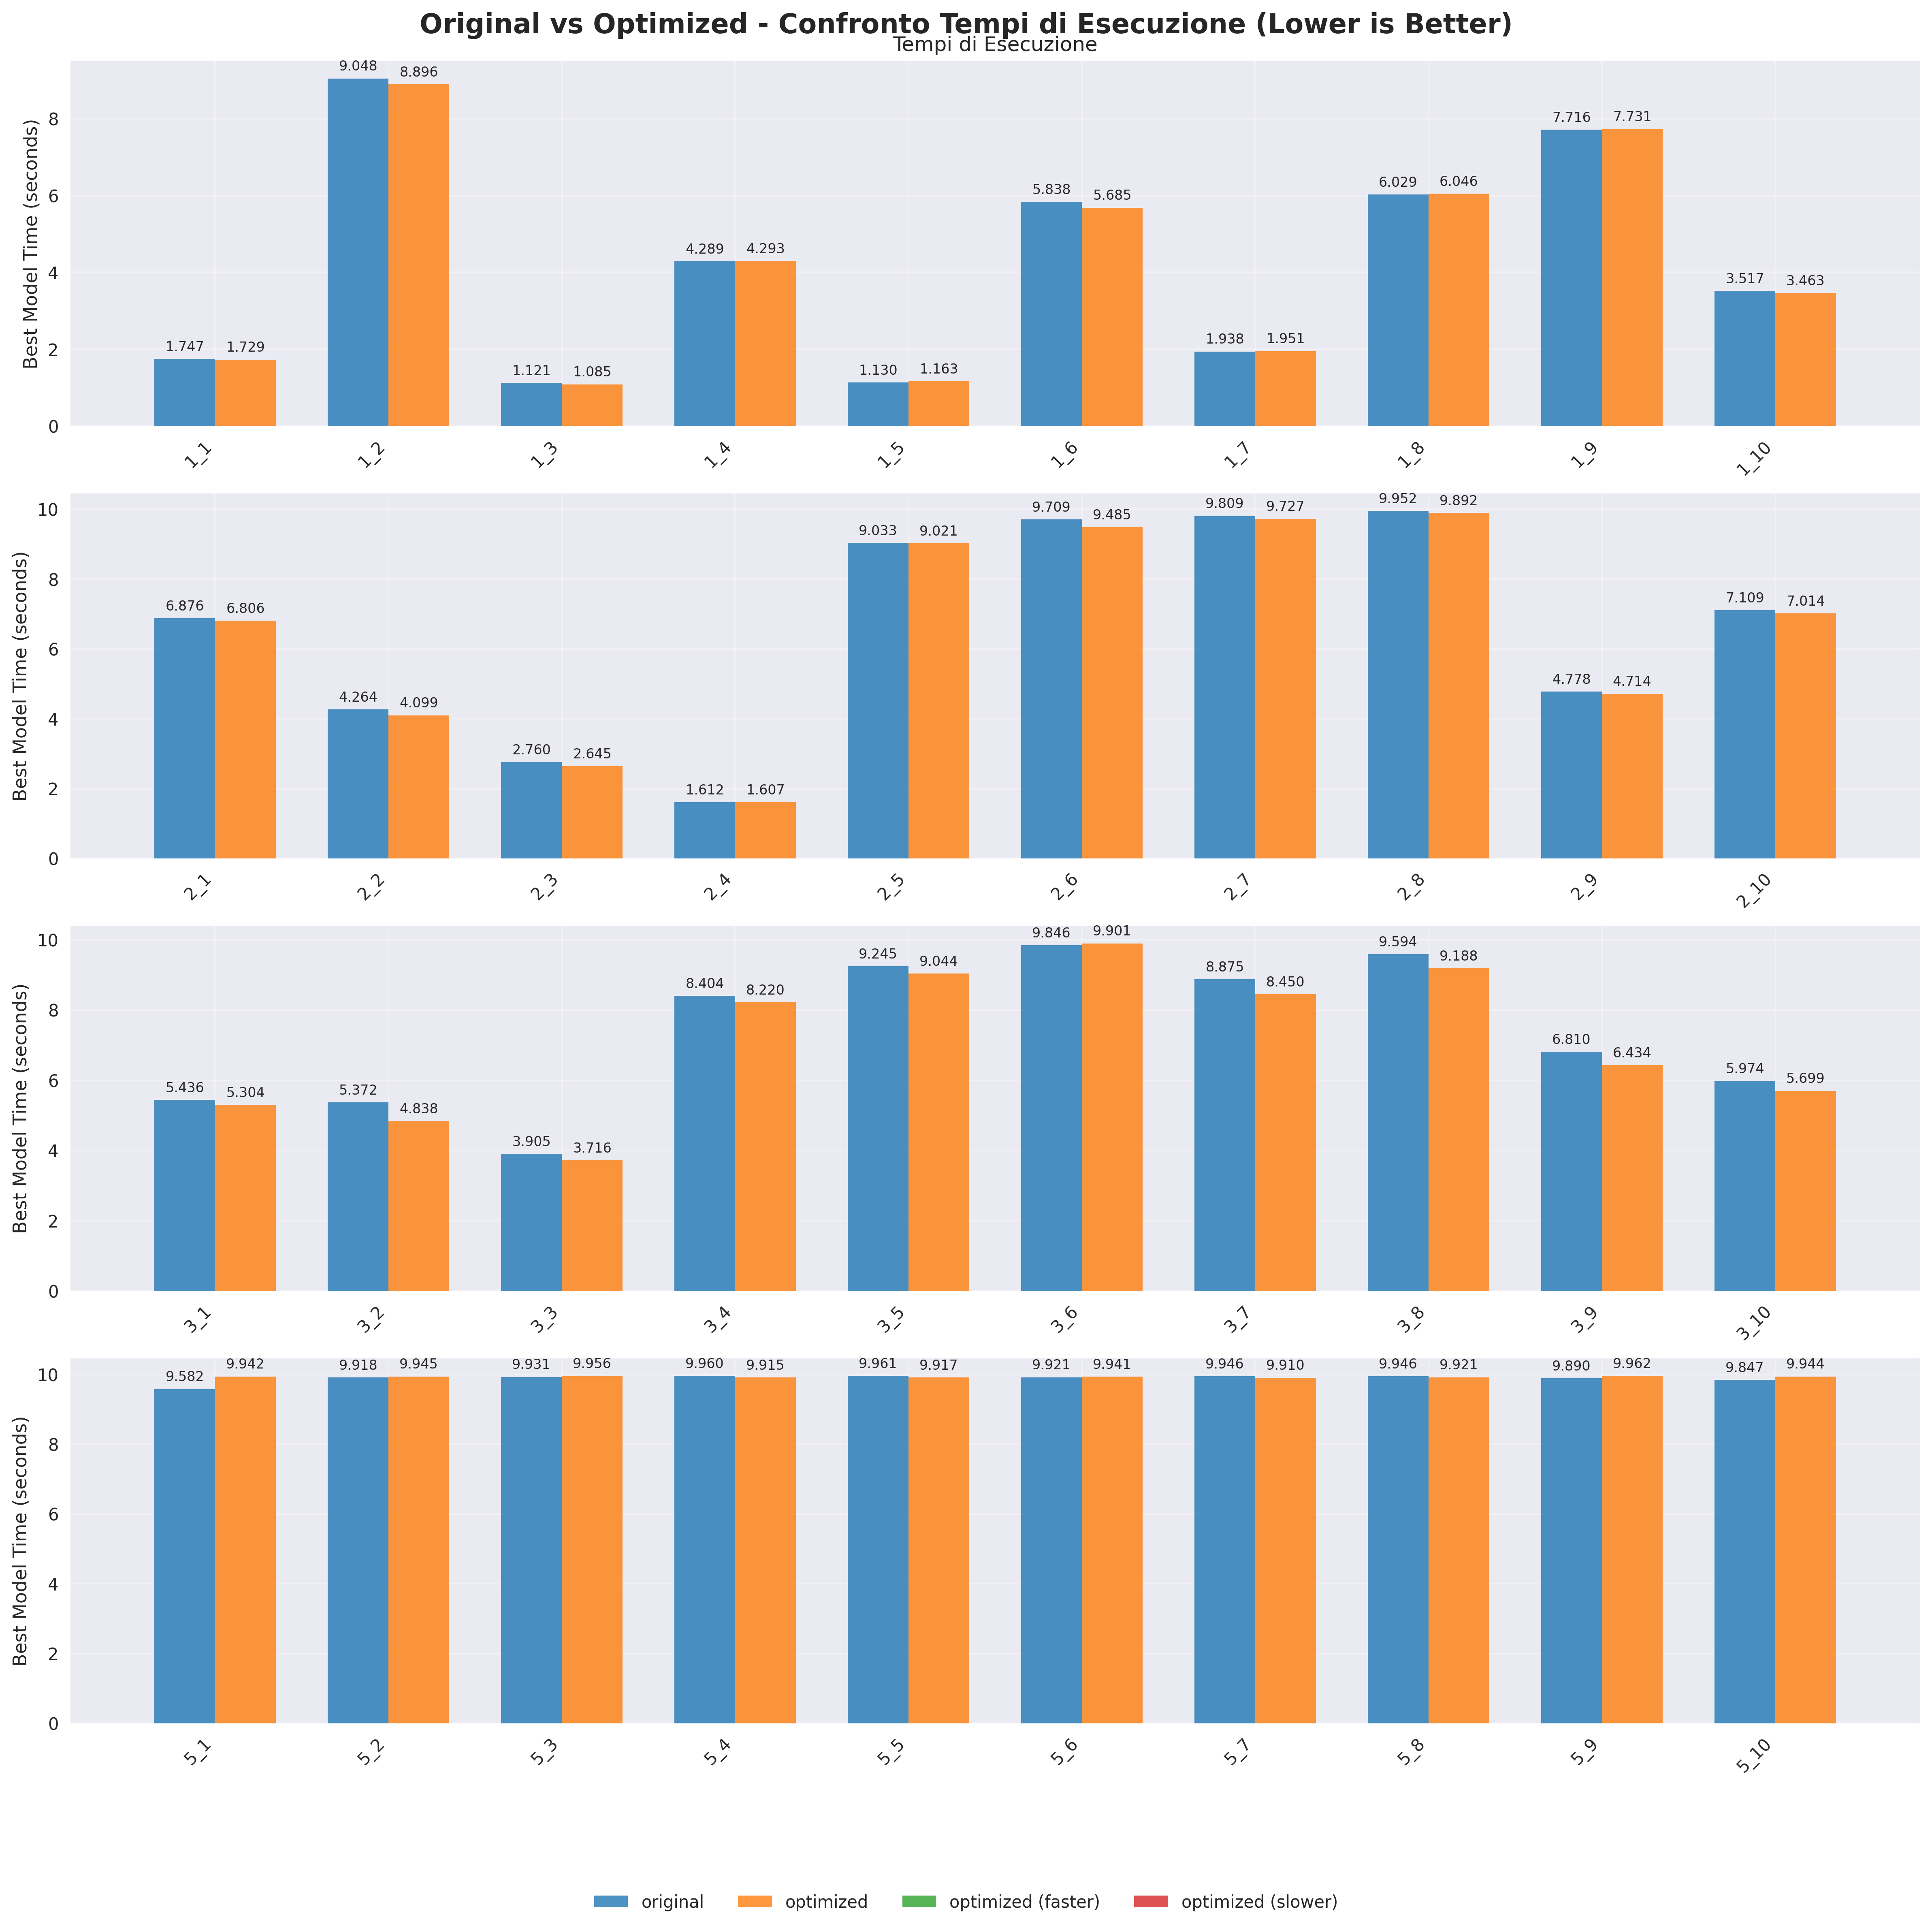
\includegraphics[width=0.8\textwidth]{time_comparison_original_vs_optimized.png}
    \caption{Execution Time Comparison: Original vs Optimized Encoding}
    \label{fig:time_orig_opt}
\end{figure}

Execution time analysis, presented in Figure \ref{fig:time_orig_opt}, reveals the temporal advantages of optimized encodings. The threshold for significant improvement is set at 2 seconds difference to filter out minor variations that may be attributed to system fluctuations.

\begin{figure}[H]
    \centering
    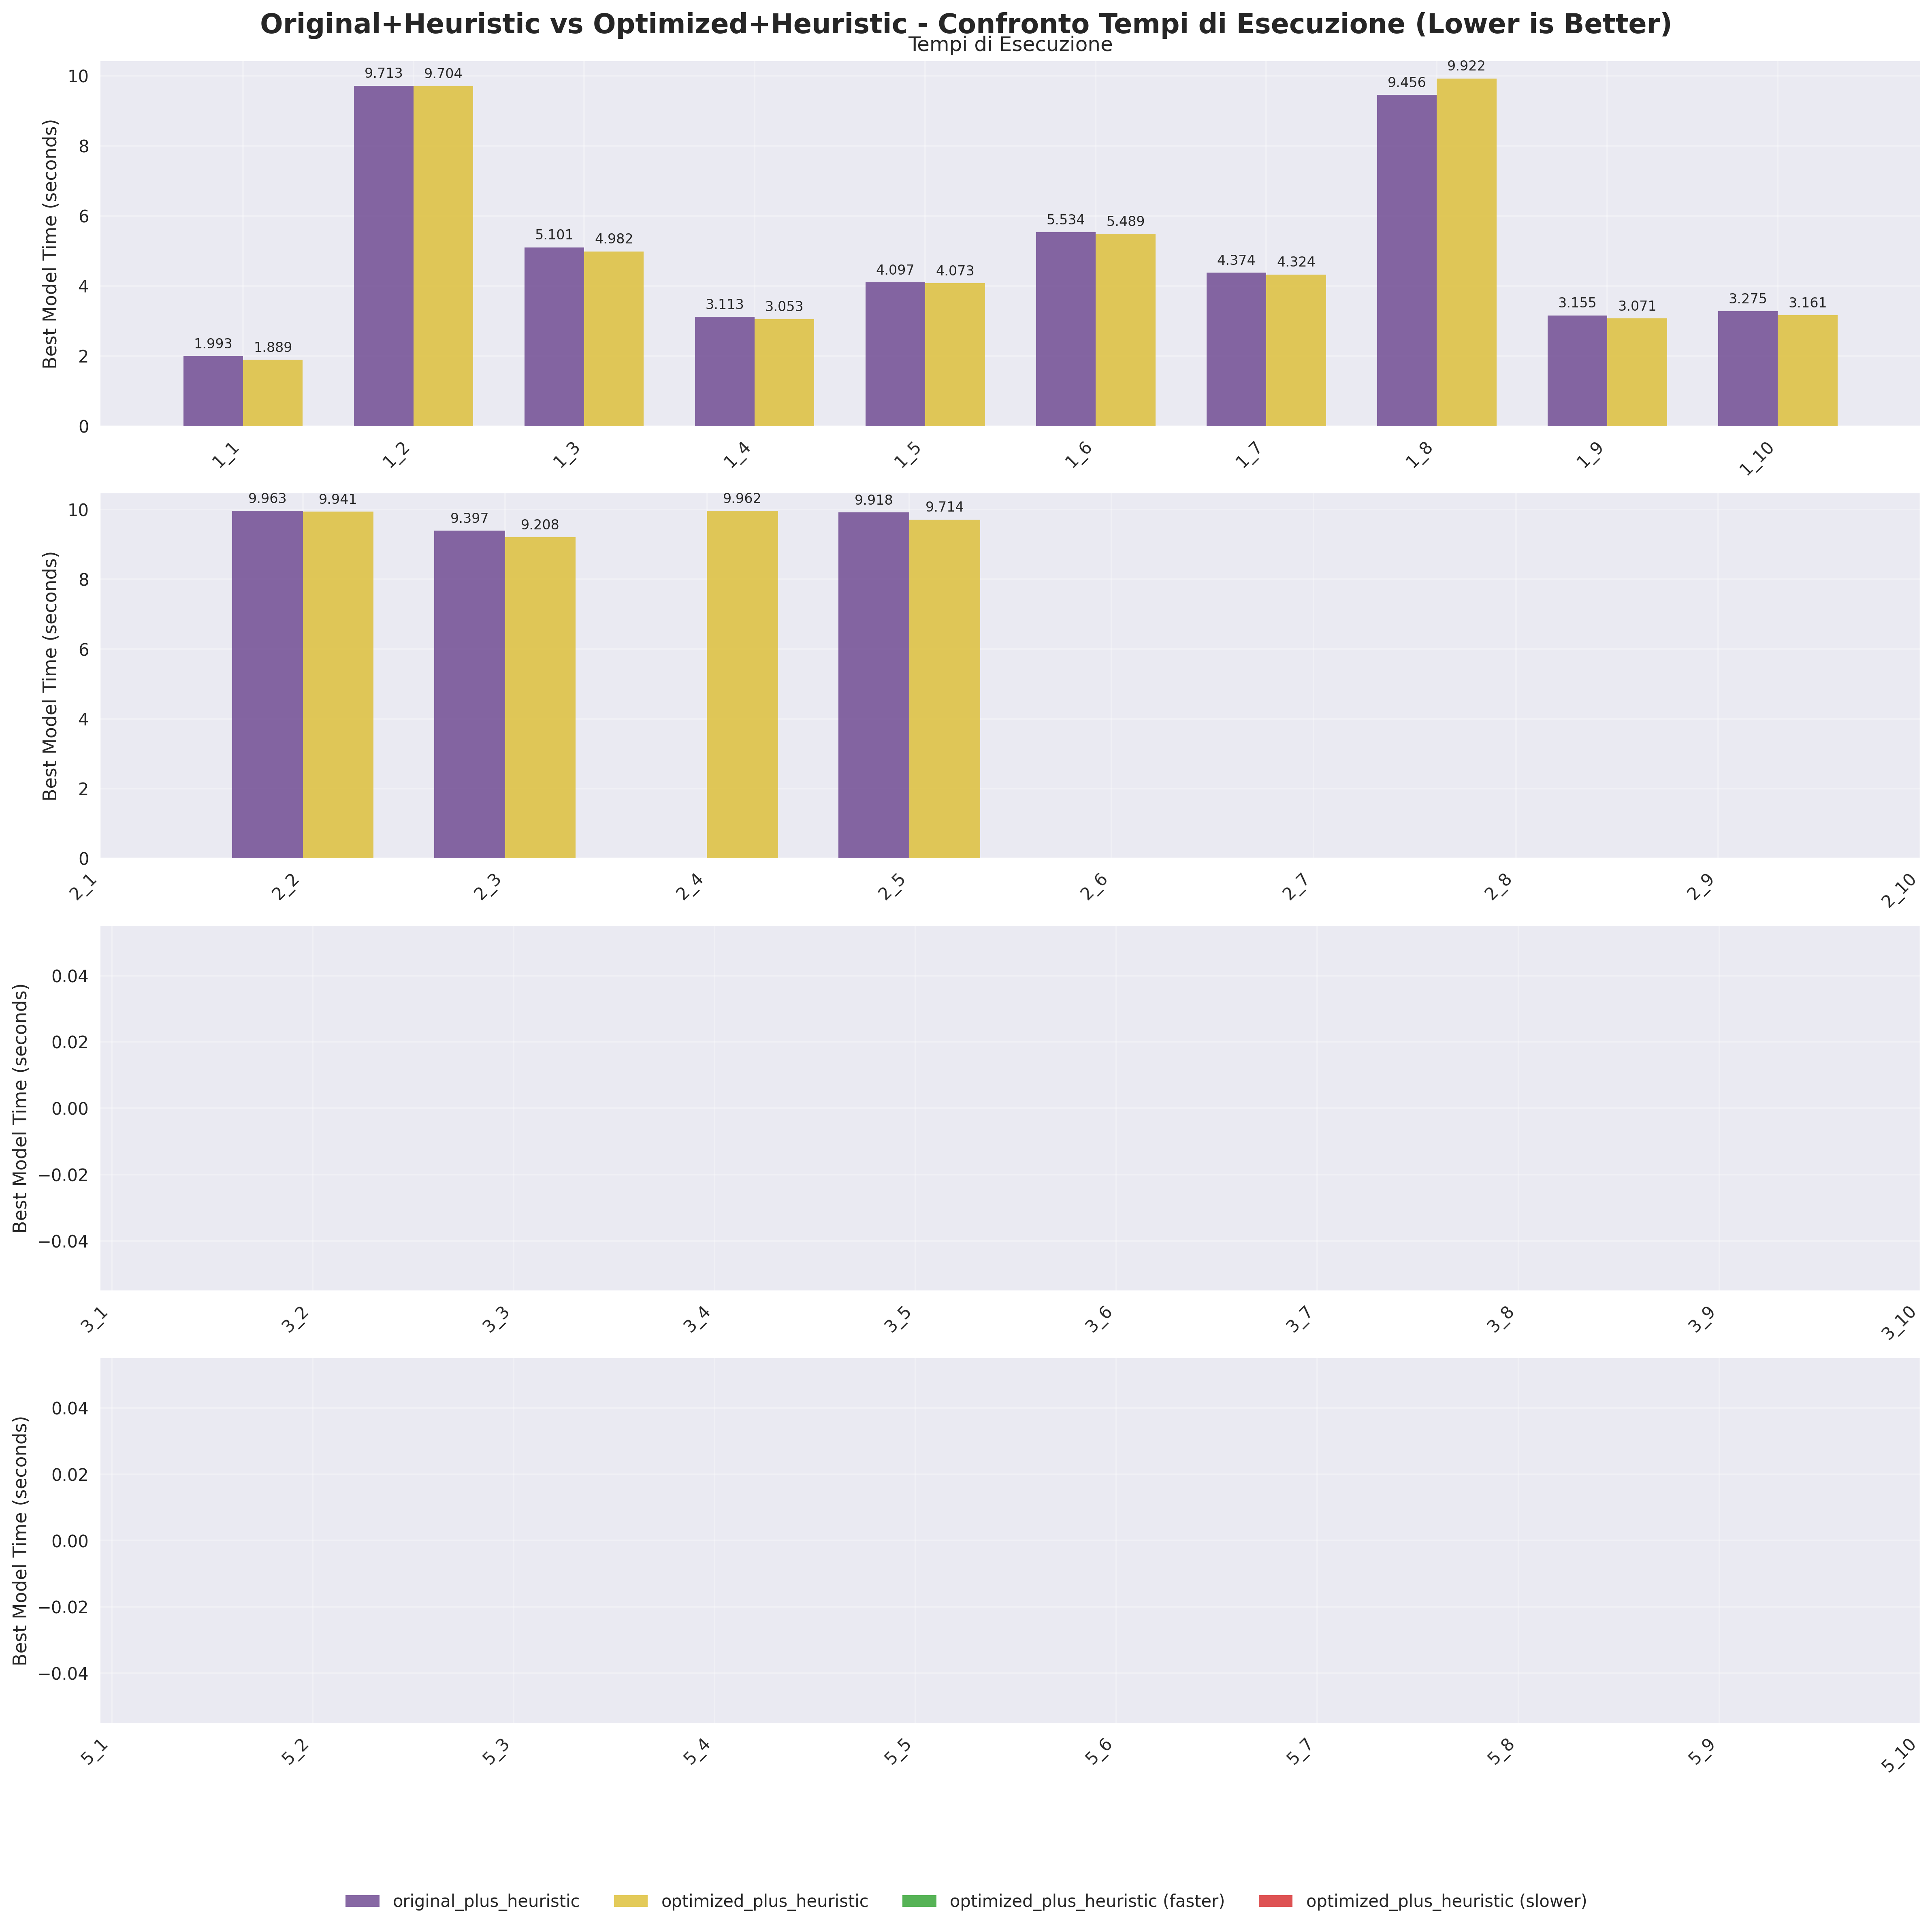
\includegraphics[width=0.8\textwidth]{time_comparison_heuristic.png}
    \caption{Execution Time Comparison: Heuristic-Enhanced Encodings}
    \label{fig:time_heuristic}
\end{figure}

\section{Technical Implementation Details}

\subsection{Heuristic Extraction and Testing Framework}

The research methodology employed a sophisticated automated framework for heuristic evaluation. The system utilizes regular expression-based parsing to extract individual heuristics from comprehensive heuristic libraries, enabling systematic evaluation of large heuristic sets without manual intervention.

The testing pipeline incorporates baseline establishment, individual heuristic assessment, and combination analysis phases. Each phase employs rigorous timing mechanisms and result validation to ensure data integrity and reproducibility of results.

\subsection{Data Collection and Analysis Pipeline}

The data collection system captures multiple performance metrics including solution costs, execution times, model counts, and solution completeness indicators. This comprehensive data collection enables multi-dimensional analysis of heuristic effectiveness.

Results are automatically processed through statistical analysis pipelines that generate comparative visualizations and performance summaries. The system employs color-coded indication schemes to highlight performance improvements, degradations, and timeout conditions across different test configurations.

\section{Key Findings and Implications}

\subsection{Primary Research Outcomes}

The research yields several significant findings that advance our understanding of heuristic effectiveness in ASP problem solving. Most importantly, heuristics demonstrate substantially greater impact on global optimization discovery than on initial solution finding, with speedup factors reaching 6.65 times baseline performance.

The generalizability of heuristic improvements across diverse problem instances suggests that well-designed heuristic strategies can provide robust performance enhancements for broad classes of ASP problems. However, the research also reveals that heuristic effectiveness is highly dependent on problem characteristics and encoding strategies.

\subsection{Practical Applications}

These findings have immediate practical implications for ASP solver deployment in real-world applications. Organizations dealing with complex combinatorial optimization problems can expect significant performance improvements through strategic heuristic implementation, particularly when global optimality is required.

The identification of effective heuristic combinations provides practitioners with proven strategies that can be immediately applied to similar problem domains. The research also establishes performance benchmarks that can guide future heuristic development efforts.

\subsection{Limitations and Future Work}

While the research provides comprehensive insights into heuristic effectiveness, several limitations warrant consideration. The timeout constraint of 180 seconds may not reflect the requirements of all real-world applications, and the specific problem domain may limit the generalizability of findings to other ASP application areas.

Future research directions include extending the analysis to longer timeout periods, evaluating heuristic effectiveness across different problem domains, and investigating dynamic heuristic selection strategies that adapt to problem characteristics during solving.

\section{Conclusions}

This comprehensive analysis of heuristic strategies in Answer Set Programming demonstrates the significant potential for performance optimization through targeted heuristic application. The research establishes that while heuristics may not dramatically improve initial solution discovery, they provide substantial advantages in achieving global optimality.

The identification of effective heuristic combinations, coupled with the demonstration of their generalizability across diverse problem instances, provides valuable guidance for practitioners seeking to optimize ASP solver performance. The systematic methodology developed for this research also contributes a reusable framework for future heuristic evaluation studies.

The findings support the continued investment in heuristic research for ASP applications, with particular emphasis on combinations that balance computational overhead with optimization effectiveness. The evidence strongly suggests that heuristic-enhanced ASP solving represents a mature and practical approach for addressing complex combinatorial optimization challenges.

\section{References and Technical Appendices}

\subsection{Implementation Resources}

The complete implementation framework, including all scripts, configuration files, and data processing utilities, is available through the project repository. The automated testing pipeline can be adapted for similar research endeavors or practical deployments.

\subsection{Statistical Analysis Details}

Detailed statistical analyses, including confidence intervals, significance testing, and variance analysis, support the conclusions presented in this research. The comprehensive dataset enables further statistical exploration and meta-analysis across different problem characteristics.

\end{document}